\section{System Overview}
This section provides a system perspective of AZ-SMART.  The system
is a distributed configuration as depicted in Figure
\ref{figSystem}, in which there are possibly different servers for
the geodatabase (ArcSDE and MS SQL Server), the land use model
(OPUS), the travel model, and potentially a web server (using ArcIMS
or its successor).  Initially we expect that OPUS and ArcGIS will be
running strictly on the same machine.

The interface between ArcGIS and OPUS will be integrated through the ArcGIS user interface (described in more detail in the subsection on
user interface).  There may be situations in which a user wishes to run an OPUS client independently of ArcGIS, for example when focusing
on model estimation, or at times when controlling simulation runs, or in the use of a fully automated batch simulation linking the land
use and travel model systems.  Similarly, a user might want to have multiple OPUS Clients on different machines, but share an OPUS Server
on another machine, to take advantage of a fast server, for example.  The interface between OPUS clients and servers would use networking
infrastructure, though there may be no need for this infrastructure during the first phase of this project.

In the first phase, the OPUS client and server will be on the same
machine as an ArcGIS workstation, with multiple installations, one
per user (or machine).  Data will be shared via the geodatabase, and
if desired also through a drive that is mapped from each of the
clients to share the cache directory containing simulation results.

\begin{figure}[h]
\begin{center}
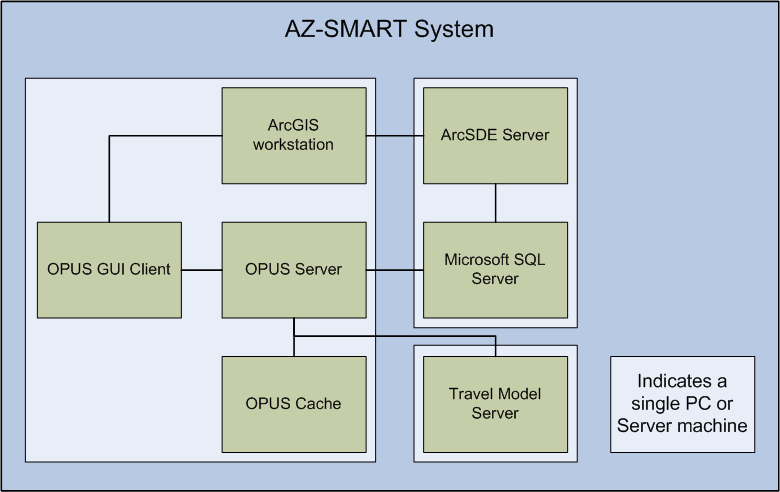
\includegraphics[scale=0.5]{figures/AZ-SMART_system_diagram.png}
\caption{AZ-SMART System Architecture}
\label{figSystem}
\end{center}
\end{figure}

%\newpage
